\hypertarget{appendix-68f22c734be3}{}
\section*{07 - Matrices, Transforms and Quaternions - Visual Recall}
\section{Matrices, Transforms and Quaternions --- Visual Recall}\label{matrices-transforms-and-quaternions-visual-recall}

Companion to \href{Continuous\%20Notes/Computing\%20Foundations\%20-\%20From\%20Bits\%20to\%20C++\%20and\%20Systems\%20APIs\#Keep\%20the\%20promises\%20visible\%20while\%20moving\%20between\%20representations}{the Phase 7 teaching story}. Start with the short route, reconstruct a worked figure, then follow its link when an assumption or definition is missing. Six excerpts supply 84 numbered lessons; the affine bridge is reconstruction, and Parts 635--650 remain source gaps.

\subsection{The short route}\label{the-short-route}

\pandocbounded{\includegraphics[keepaspectratio,alt={Diagram}]{/Users/swayamsingal/Library/Mobile Documents/iCloud~md~obsidian/Documents/Master/Book Production/AllMight Codex/QA/print-reference-dedup/assets/print/03b38c7eb65bb64e2bd1150c0250d97edc942be0f60b74650125121a64dde4f3.pdf}}

\textbf{Convention card:} active right-handed rotations; column vectors; \(y=Mx\); rightmost operation first; code angles in radians; Hamilton quaternion components \((w,x,y,z)\). Row-major storage does not choose any of those mathematical conventions.

{\def\LTcaptype{none} % do not increment counter
\begin{longtable}[]{@{}
  >{\raggedright\arraybackslash}p{(\linewidth - 4\tabcolsep) * \real{0.3333}}
  >{\raggedright\arraybackslash}p{(\linewidth - 4\tabcolsep) * \real{0.3333}}
  >{\raggedright\arraybackslash}p{(\linewidth - 4\tabcolsep) * \real{0.3333}}@{}}
\toprule\noalign{}
\begin{minipage}[b]{\linewidth}\raggedright
Topic
\end{minipage} & \begin{minipage}[b]{\linewidth}\raggedright
Shortest useful rule
\end{minipage} & \begin{minipage}[b]{\linewidth}\raggedright
Figure or explanation
\end{minipage} \\
\midrule\noalign{}
\endhead
\bottomrule\noalign{}
\endlastfoot
Meaning & A rectangular table becomes a map only after input/output bases and roles are fixed. Columns are input-basis images. & \href{Continuous\%20Notes/Computing\%20Foundations\%20-\%20From\%20Bits\%20to\%20C++\%20and\%20Systems\%20APIs\#Figure\%20M1\%20-\%20Coordinates\%20weight\%20the\%20new\%20basis\%20directions/}{M1: weighted columns} \\
Shape & \((m\times k)(k\times n)\) yields \(m\times n\); shared dimensions must match. Addition needs equal shape. & \href{Continuous\%20Notes/Computing\%20Foundations\%20-\%20From\%20Bits\%20to\%20C++\%20and\%20Systems\%20APIs\#Combining\%20rules\%20explains\%20the\%20multiplication\%20law/}{Derive the product} \\
Composition & \(ABx\) applies \(B\) first. Noncommutative order is separate from associative grouping; floating-point regrouping can change bits. & \href{Continuous\%20Notes/Computing\%20Foundations\%20-\%20From\%20Bits\%20to\%20C++\%20and\%20Systems\%20APIs\#Figure\%20M2\%20-\%20The\%20same\%20operations\%20give\%20different\%20results\%20in\%20different\%20orders/}{M2: two orders} \\
Rotations & Derive columns from rotated axes. For \(R_y\), rotate the oriented pair \((z,x)\), then restore \((x,y,z)\) order. & \href{Continuous\%20Notes/Computing\%20Foundations\%20-\%20From\%20Bits\%20to\%20C++\%20and\%20Systems\%20APIs\#The\%20oriented\%20plane\%20explains\%20the\%20Y-rotation\%20signs/}{Axis derivation and values} \\
Structure & \((AB)^T=B^TA^T\); \(A=(A+A^T)/2+(A-A^T)/2\). Trace is similarity-invariant, not a full map identifier. & \href{Continuous\%20Notes/Computing\%20Foundations\%20-\%20From\%20Bits\%20to\%20C++\%20and\%20Systems\%20APIs\#Transpose\%20lets\%20us\%20compare\%20measurements\%20and\%20structure/}{Transpose, symmetry and trace} \\
Determinant & Magnitude = volume scale; sign = orientation; zero = rank loss for square maps. It does not measure conditioning alone. & \href{Continuous\%20Notes/Computing\%20Foundations\%20-\%20From\%20Bits\%20to\%20C++\%20and\%20Systems\%20APIs\#Figure\%20M3\%20-\%20Three\%20different\%20questions\%20answered\%20by\%20one\%20determinant/}{M3: determinant questions} \\
Inversion & Cofactors explain a formula; pivoted elimination explains an algorithm. Solve directly when the inverse itself is unnecessary. & \href{Continuous\%20Notes/Computing\%20Foundations\%20-\%20From\%20Bits\%20to\%20C++\%20and\%20Systems\%20APIs\#Row\%20reduction\%20makes\%20the\%20inverse\%20observable/}{Full elimination trace} \\
Sensitivity & \(\kappa(A)=\|A\|\|A^{-1}\|\) in a compatible norm. Stable code cannot restore information lost to input uncertainty. & \href{Continuous\%20Notes/Computing\%20Foundations\%20-\%20From\%20Bits\%20to\%20C++\%20and\%20Systems\%20APIs\#Figure\%20M4\%20-\%20Uncertainty\%20can\%20be\%20amplified\%20by\%20a\%20reversible\%20map/}{M4: perturbed observation} \\
Point/vector & Affine points receive \(Ap+t\); displacements receive \(Av\). Homogeneous \(w=1\) and \(w=0\) expose the distinction. & \href{Continuous\%20Notes/Computing\%20Foundations\%20-\%20From\%20Bits\%20to\%20C++\%20and\%20Systems\%20APIs\#Figure\%20M5\%20-\%20The\%20same\%20frame\%20moves\%20a\%20point\%20and\%20redirects\%20a\%20displacement/}{M5: two roles} \\
Frames & \(F_C^{-1}F_B\) converts B-coordinates to C-coordinates. The camera view is the inverse camera pose. & \href{Continuous\%20Notes/Computing\%20Foundations\%20-\%20From\%20Bits\%20to\%20C++\%20and\%20Systems\%20APIs\#Coordinates\%20can\%20change\%20while\%20the\%20geometric\%20object\%20stays\%20still/}{Active/passive and frame conversion} \\
Projection & Clip retains \(w\); NDC divides by valid \(w\). Clipping, depth range and backend conventions remain explicit. & \href{Continuous\%20Notes/Computing\%20Foundations\%20-\%20From\%20Bits\%20to\%20C++\%20and\%20Systems\%20APIs\#Figure\%20M6\%20-\%20Follow\%20one\%20point\%20through\%20named\%20spaces/}{M6: complete point walk} \\
Normals & \(n'=A^{-T}n\) preserves zero action on transformed tangents. Normalize only after a valid transformation. & \href{Continuous\%20Notes/Computing\%20Foundations\%20-\%20From\%20Bits\%20to\%20C++\%20and\%20Systems\%20APIs\#A\%20normal\%20transforms\%20as\%20a\%20measurement\%20that\%20must\%20still\%20vanish\%20on\%20tangents/}{Proof and counterexample} \\
Layout & Logical width is not physical stride. Real arrays provide array bounds; views borrow both layout and lifetime. & \href{Continuous\%20Notes/Computing\%20Foundations\%20-\%20From\%20Bits\%20to\%20C++\%20and\%20Systems\%20APIs\#Figure\%20M7\%20-\%20A\%20submatrix\%20keeps\%20the\%20parent's\%20physical\%20stride/}{M7: subview addresses} \\
Performance & SIMD, loop order and tiling change reuse and rounding. Measure hardware/workload; algebra alone supplies no speedup. & \href{Continuous\%20Notes/Computing\%20Foundations\%20-\%20From\%20Bits\%20to\%20C++\%20and\%20Systems\%20APIs\#SIMD\%20and\%20loop\%20order\%20change\%20the\%20execution\%20schedule,\%20not\%20the\%20matrix\%20question/}{Reuse and loop trace} \\
Quaternion & Hamilton product = scalar/dot part + weighted vectors/cross part. Unit \(q\) permits inverse-by-conjugate. & \href{Continuous\%20Notes/Computing\%20Foundations\%20-\%20From\%20Bits\%20to\%20C++\%20and\%20Systems\%20APIs\#Figure\%20M8\%20-\%20One\%20orientation,\%20several\%20checkable\%20actions/}{M8: axis to action} \\
Half-angle & \(q=(\cos(\theta/2),a\sin(\theta/2))\) for unit axis. Two-sided action produces the full angle; \(q\) and \(-q\) share orientation. & \href{Continuous\%20Notes/Computing\%20Foundations\%20-\%20From\%20Bits\%20to\%20C++\%20and\%20Systems\%20APIs\#Derive\%20the\%20axis-angle\%20mapping\%20by\%20deriving\%20its\%20action/}{Sandwich derivation} \\
Conversion & Quaternion↔matrix tests compare basis actions; near \(180^\circ\) recover a large component. Reject scale/shear/reflection as rotation inputs. & \href{Continuous\%20Notes/Computing\%20Foundations\%20-\%20From\%20Bits\%20to\%20C++\%20and\%20Systems\%20APIs\#Recover\%20a\%20large\%20component\%20instead\%20of\%20dividing\%20by\%20a\%20nearly-zero\%20one/}{Stable branches} \\
Interpolation & Sign-align endpoints. NLERP normalizes the chord; SLERP advances on the great circle. Small-angle fallback needs a policy. & \href{Continuous\%20Notes/Computing\%20Foundations\%20-\%20From\%20Bits\%20to\%20C++\%20and\%20Systems\%20APIs\#Figure\%20M9\%20-\%20Choose\%20a\%20representative\%20before\%20choosing\%20a\%20path/}{M9: path selection} \\
Euler & Axis sequence is part of the type contract. Gimbal lock is a singular coordinate chart; original angle history cannot be recovered. & \href{Continuous\%20Notes/Computing\%20Foundations\%20-\%20From\%20Bits\%20to\%20C++\%20and\%20Systems\%20APIs\#Euler\%20coordinates\%20remain\%20useful\%20when\%20their\%20chart\%20is\%20explicit/}{Substitute the singular pitch} \\
Rigid dual & \(q_d=(0,t)q_r/2\); require \(\|q_r\|=1\) and \(q_r\cdot q_d=0\). Do not normalize the two halves independently. & \href{Continuous\%20Notes/Computing\%20Foundations\%20-\%20From\%20Bits\%20to\%20C++\%20and\%20Systems\%20APIs\#Two\%20coupled\%20constraints\%20make\%20the\%20eight\%20coefficients\%20a\%20rigid\%20motion/}{Study constraint and recovery} \\
TRS/cache & Local TRS is useful authoring data; full affine world products may contain shear. Dirty flags record dependency invalidation. & \href{Continuous\%20Notes/Computing\%20Foundations\%20-\%20From\%20Bits\%20to\%20C++\%20and\%20Systems\%20APIs\#Figure\%20M10\%20-\%20Representation\%20follows\%20the\%20permitted\%20operation/}{M10: choose representation} · \href{Continuous\%20Notes/Computing\%20Foundations\%20-\%20From\%20Bits\%20to\%20C++\%20and\%20Systems\%20APIs\#Figure\%20M11\%20-\%20Invalidate\%20the\%20values\%20that\%20actually\%20depend\%20on\%20the\%20edit/}{M11: cache dependencies} \\
\end{longtable}
}

\subsection{Four experiments to reconstruct without the chapter}\label{four-experiments-to-reconstruct-without-the-chapter}

\begin{enumerate}
\def\labelenumi{\arabic{enumi}.}
\tightlist
\item
  Send \((4,2)\) through columns \((2,1)\) and \((-1,3)\). Obtain \((6,10)\) by column contributions and row sums. Explain why changing storage cannot change that answer.
\item
  Compare observations \((2,2.001)\) and \((2,2.002)\) for \(A=\begin{bmatrix}1&1\\1&1.001\end{bmatrix}\). Recover \((1,1)\) versus \((0,2)\) and identify the source of uncertainty.
\item
  For \(q_Z=(\sqrt2/2,0,0,\sqrt2/2)\), rotate X to Y. Then use \(2q_Z\): true inverse still gives Y, conjugate sandwich gives four times Y, and the unit-optimized formula is outside its contract.
\item
  Compare the columns of \(S R_{45^\circ}\) with \(S=\operatorname{diag}(2,1)\). Their dot is \(-3/2\), proving that the result is not an orthogonal rotation times diagonal scale.
\end{enumerate}

\textbf{Teaching check:} explain every coefficient, space and failure result before running \href{Continuous\%20Notes/Computing\%20Foundations\%20-\%20From\%20Bits\%20to\%20C++\%20and\%20Systems\%20APIs\#A\%20complete\%20scalar\%20laboratory\%20makes\%20the\%20contracts\%20observable}{the standalone C++ laboratory}. Written coverage and successful tests do not measure personal mastery.

\href{}{Source ledger and gap (01-Foundations-I, appendix-fd090d982a15 § Phase 7 - Parts 601-700)} · \href{Continuous\%20Notes/Computing\%20Foundations\%20-\%20From\%20Bits\%20to\%20C++\%20and\%20Systems\%20APIs\#Phase\%207\%20-\%20Transform\%20reconstruction\%20proofs}{Derivations} · \href{}{Tracebook (01-Foundations-I, appendix-92ff77d4dfdc § Phase 7 - The moving-panel tracebook)} · \hyperref[appendix-4ad47bdd269a]{Dependency Map}

\subsection{Added retrieval prompt}\label{added-retrieval-prompt}

Project onto y=x: standard matrix \url{1/2,1/2\%5D,\%5B1/2,1/2}, aligned-basis matrix diag(1,0); explain why P squared equals P. \href{Continuous\%20Notes/Computing\%20Foundations\%20-\%20From\%20Bits\%20to\%20C++\%20and\%20Systems\%20APIs\#A\%20linear\%20rule\%20is\%20determined\%20by\%20its\%20basis\%20images}{Rebuild both descriptions}.

\begin{figure}
\centering
\pandocbounded{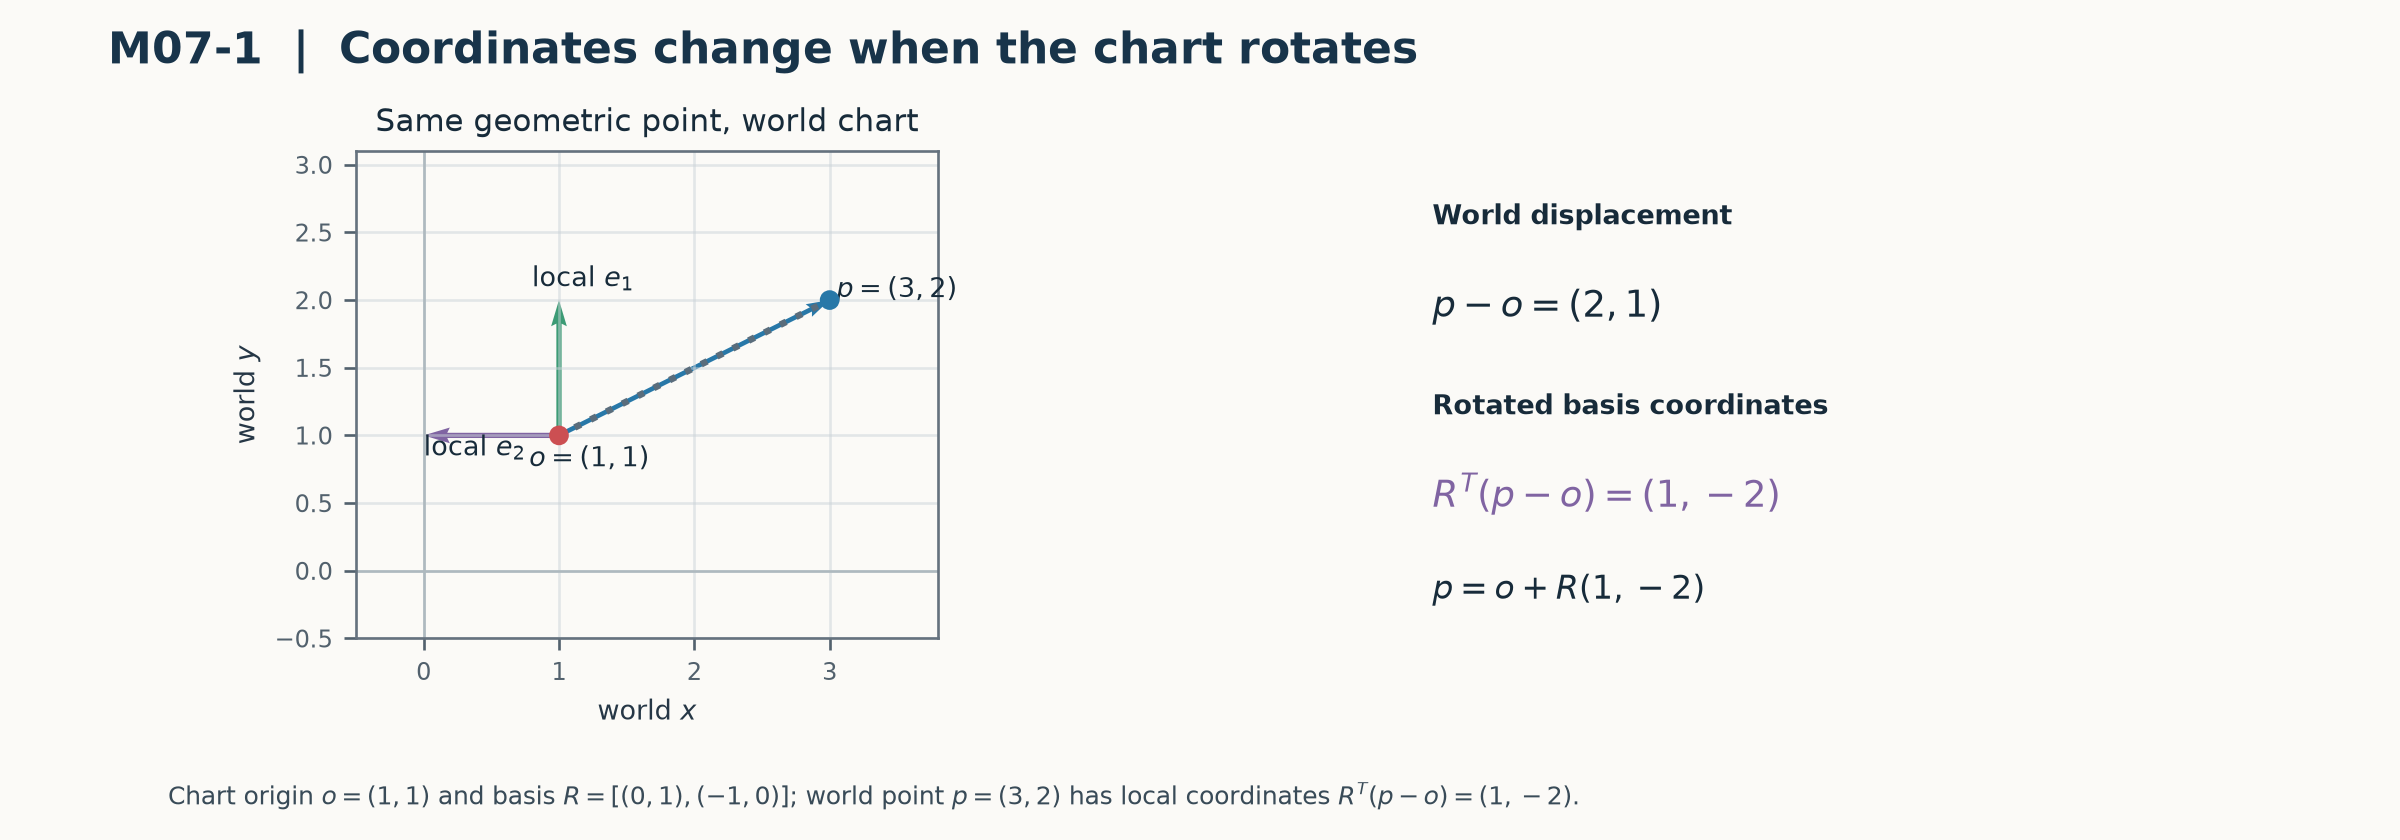
\includegraphics[keepaspectratio,alt={Visual Recall/Math Foundations/M07-1\_rotated-coordinate-chart.png}]{Visual Recall/Math Foundations/M07-1_rotated-coordinate-chart.png}}
\caption{Visual Recall/Math Foundations/M07-1\_rotated-coordinate-chart.png}
\end{figure}

\textbf{M07-1. A point expressed in a rotated local chart.} For the quarter-turn basis at (1,1), point (3,2) has local coordinates (1,-2) and reconstructs the original point.
